% tikzpic.tex
\documentclass[crop,tikz]{standalone}% 'crop' is the default for v1.0, before it was 'preview'

%\usetikzlibrary{...}% tikz package already loaded by 'tikz' option
\usetikzlibrary{shapes.geometric}
\usetikzlibrary{arrows.meta}
\usetikzlibrary{positioning}
\usetikzlibrary{calc}

\usepackage[outline]{contour}

\usepackage{rotating}

\begin{document}

\def\layersep{1.5cm}
\definecolor{correctLabel}{rgb}{0.8392156862745098,0.15294117647058825,0.1568627450980392}
\definecolor{incorrectLabel}{rgb}{0.12156862745098039, 0.4666666666666667, 0.7058823529411765}

\definecolor{mplColoursC0}{rgb}{0.12156862745098039, 0.4666666666666667, 0.7058823529411765}
\definecolor{mplColoursC1}{rgb}{1.0, 0.4980392156862745, 0.054901960784313725}
\definecolor{mplColoursC2}{rgb}{0.17254901960784313, 0.6274509803921569, 0.17254901960784313}
\definecolor{mplColoursC3}{rgb}{0.8392156862745098, 0.15294117647058825, 0.1568627450980392}

\def\inputshadeIa{100}
\def\inputshadeIb{15}
\def\inputshadeIc{0}
\def\inputshadeId{85}
\def\inputshadeIe{50}

\begin{tikzpicture}[
            % font={\sffamily \small},
            scale=1.,
            >=latex,
            transform shape,
        ]
        \pgfdeclarelayer{background layer}
        \pgfsetlayers{background layer,main}
        \draw[use as bounding box,inner sep=0pt, anchor=north west] node {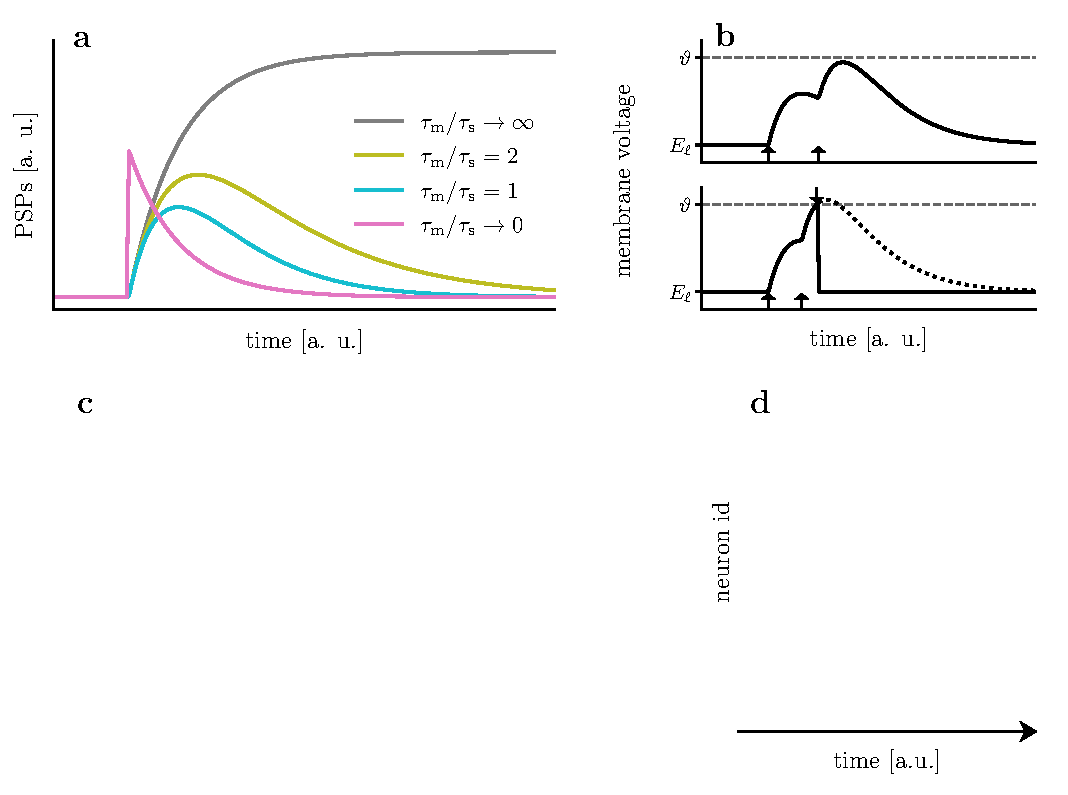
\includegraphics[width=\textwidth]{../../fig/figSetup.pdf}};

       \node[inner sep=0pt, anchor=north west] (whitehead) at (0.35, -4.45)
       {
		   \begin{turn}{90}
               			\begin{tikzpicture}[
				shorten >=0.05pt,
				->,
				draw=black,
				node distance=\layersep,
				scale=1.2,
				transform shape]
				\tikzstyle{every pin edge}=[<-,shorten <=0.5pt]
				\tikzstyle{neuron}=[circle,draw=black,minimum size=17pt,inner sep=0pt, line width=1.0pt]
				\tikzstyle{triangle} = [neuron, regular polygon, regular polygon sides=3,rotate=-90];
				\tikzstyle{input neuron}=[neuron, rectangle, minimum size=14pt];
                \tikzstyle{input neuron-1}=[input neuron, fill=black!\inputshadeIa];
                \tikzstyle{input neuron-2}=[input neuron, fill=black!\inputshadeIb];
                \tikzstyle{input neuron-3}=[input neuron, fill=black!\inputshadeIc];
                \tikzstyle{input neuron-4}=[input neuron, fill=black!\inputshadeId];
                \tikzstyle{input neuron-5}=[input neuron, fill=black!\inputshadeIe];
				\tikzstyle{hidden neuron}=[neuron, draw=gray];
				\tikzstyle{label neuron}=[neuron, triangle, draw=none];
				\tikzstyle{label neuron-1}=[label neuron, fill=mplColoursC0, ];
				\tikzstyle{label neuron-2}=[label neuron, fill=mplColoursC3, ];
				\tikzstyle{label neuron-3}=[label neuron, fill=mplColoursC2, ];
				\tikzstyle{label neuron-4}=[label neuron, fill=mplColoursC1, ];
				\tikzstyle{annot} = [text width=4em, text centered]
				\tikzstyle{connection} = [line width=0.8pt, -{Latex[length=6.0pt, width=4.0pt]}, draw=black!80]

				\def\numInputs{5}
				\def\numHidden{6}
				\def\numLabel{3}
                \def\yshiftInput{1.0}
                \def\yshiftHidden{1.5}
                \def\yshiftLabel{0.0}

				% Draw the input layer nodes
				\foreach \name / \y in {1,...,\numInputs}
				% This is the same as writing \foreach \name / \y in {1/1,2/2,3/3,4/4}
					\path[yshift=\yshiftInput cm, anchor=center]
                        node[input neuron-\name, anchor=center] (I-\name) at (0, -\y cm) {};

				% Draw the hidden layer nodes
				\foreach \name / \y in {1,...,\numHidden}
					\path[yshift=\yshiftHidden cm, anchor=center]
						node[hidden neuron] (H-\name) at (\layersep, -\y cm) {};

				% Draw the label layer node
				\foreach \name / \y in {1,...,\numLabel}
					\path[yshift=\yshiftLabel cm]
						node[label neuron-\name] (L-\name) at (2 *\layersep, -\y cm) {};
				% \node[label neuron,pin={[pin edge={->}]right:Output},  of=H-3] (L) {};

				% Connect every node in the input layer with every node in the
				% hidden layer.
				\foreach \source in {1,...,\numInputs}
					\foreach \dest in {1,...,\numHidden}
						% \path[connection] (I-\source) edge (H-\dest);
						\draw[connection] (I-\source) --++ (H-\dest);

				% Connect every node in the hidden layer with the label layer
				\foreach \source in {1,...,\numHidden}
					\foreach \dest in {1,...,\numLabel}
						\path[connection] (H-\source) edge (L-\dest);

				% % Annotate the layers
				% \node[annot, above of=H-\numHidden, xshift=-0.15cm, node distance=0.7cm, label={[rotate=-90](80)}] (H-l) {};
				% \node[annot, left of=H-l, label={[rotate=-90](49)}] (I-l) {};
				% \node[annot, right of=H-l, label={[rotate=-90](4)}] (L-l) {};
			\end{tikzpicture}


		\end{turn}
	};
       \node[inner sep=0pt, anchor=north west] (whitehead) at (8.85, -4.85)
       {
		   % \begin{turn}{90}
           			\begin{tikzpicture}[scale=2.2,x=1.3cm,y=0.9cm]

				\def\numInputs{5}
				\def\numHidden{6}
				\def\numLabel{3}

				\def\spikesHidden{{
                        % 0.4, 0.4, 0.4, 0.4, 0.4, 0.4, 
							0.4, 0.39, 
                            0.8, 0.9,
                            0.55, 0.42,
							1.105, 1.205, 0.53, 0.9,
							0.38, 0.49,
					}}
				\def\spikesLabel{{
							1.3,
							0.9,
							1.2,
							1.28
					}}

				\def\offset{0.35}

				\def\toffsetI{0.85}
				\def\toffsetH{0.10}
				\def\toffsetL{-0.35}

				\def\tScale{0.8}

				\tikzstyle{input}=[rectangle, draw=black, minimum size=2, inner sep=0pt, line width=0.4pt]
				\tikzstyle{input neuron-early}=[input, fill=black];
				\tikzstyle{input neuron-late}=[input, xshift=0.6cm * \tScale];

                \tikzstyle{input neuron-1}=[input, fill=black!\inputshadeIa, xshift=-0.6cm * \tScale * \inputshadeIa / 100]
                \tikzstyle{input neuron-2}=[input, fill=black!\inputshadeIb, xshift=-0.6cm * \tScale * \inputshadeIb / 100]
                \tikzstyle{input neuron-3}=[input, fill=black!\inputshadeIc, xshift=-0.6cm * \tScale * \inputshadeIc / 100]
                \tikzstyle{input neuron-4}=[input, fill=black!\inputshadeId, xshift=-0.6cm * \tScale * \inputshadeId / 100]
                \tikzstyle{input neuron-5}=[input, fill=black!\inputshadeIe, xshift=-0.6cm * \tScale * \inputshadeIe / 100]

				\tikzstyle{hidden neuron}=[input, circle, draw=gray];

				\tikzstyle{triangle} = [input, regular polygon, regular polygon sides=3 ];
				\tikzstyle{label neuron}=[triangle, line width=0.5pt, draw=incorrectLabel, fill=incorrectLabel];
				\tikzstyle{label neuron-1}=[label neuron, draw=mplColoursC0, fill=mplColoursC0];
				\tikzstyle{label neuron-2}=[label neuron, draw=mplColoursC3, fill=mplColoursC3];
				\tikzstyle{label neuron-3}=[label neuron, draw=mplColoursC2, fill=mplColoursC2];
				\tikzstyle{label neuron-4}=[label neuron, draw=mplColoursC1, fill=mplColoursC1];

				% Draw axes
				% \node[label={[label distance=0cm,anchor=east,xshift=-0.3cm, yshift=0.2cm, rotate=90] {\scriptsize{ $\textrm{time-to-first-spike [a.u.]}$}}}] (yaxis) at (0, 2) {};
				% \draw [-,thick] (yaxis)  [label distance=3.5cm] {}
				% 	|- (3,0) node (xaxis) {};

				% inputs
				\foreach \id in {1,...,\numInputs}
					\pgfmathsetmacro{\idCoord}{\id/10.0 + \offset}
					\pgfmathsetmacro{\tCoord}{\toffsetI * \tScale}
					\node[input neuron-\id] at (\tCoord, \idCoord) {};

				% separation
				\pgfmathsetmacro{\offset}{\offset + 0.1 * \numInputs + 0.07}
				\draw [dotted] (0.2 * \tScale, \offset) -- (1.3 * \tScale, \offset);

				\pgfmathsetmacro{\offset}{\offset + 0.13}
				% hidden spikes
				\foreach \tmpId in {1,...,\numHidden}
					\pgfmathsetmacro{\id}{\tmpId - 1}
					\pgfmathsetmacro{\idCoord}{\id/10.0 + \offset}
					\pgfmathsetmacro{\tCoord}{\spikesHidden[\id] * \tScale + \toffsetH * \tScale}
					\node[hidden neuron] (H-\id) at (\tCoord, \idCoord) {}
					;

				% separation
				\pgfmathsetmacro{\offset}{\offset +  \numHidden / 14.0 + 0.15}
				\draw [dotted] (0.2 * \tScale, \offset) -- (1.3 * \tScale, \offset);

				\pgfmathsetmacro{\offset}{\offset + 0.2}
				% label spikes
				\foreach \tmpId in {1,...,\numLabel}
					\pgfmathsetmacro{\id}{\tmpId - 1}
					\pgfmathsetmacro{\idCoord}{\id/10.0 + \offset}
					\pgfmathsetmacro{\tCoord}{\spikesLabel[\id] * \tScale + \toffsetL * \tScale}
					\node[label neuron-\tmpId] (L-\id) at (\tCoord, \idCoord) {}
					;

			\end{tikzpicture}


		% \end{turn}
	   };

    %    \node[inner sep=0pt] (whitehead) at (11.5,-0.6)
    %    {
	% 	    \includegraphics[height=.07\textwidth,angle=90]{HICANN_downscaled.jpg}
	% 	};
    %    \node[inner sep=0pt] (whitehead) at (11.6,-1.7)
    %    {
	%    		% \includegraphics[width=.08\textwidth]{wafershiny.png}
	% 	};


  \end{tikzpicture}
\end{document}
